\section{MLP vs RNN}
Confronteremo ora i risultati sperimentali ottenuti
dai modelli basati su MLP e RNN. Per farlo andremo a prendere i risultati
ottenuti sul dataset di testing mostrati in Sezione~\ref{sec:mlpeval} e \ref{sec:rnneval}, computeremo le differenze tra ground tuth e predizione
del modello ed andremo a confrontare le curve prodotte mettendo quindi in
evidenza gli errori commessi dalle due reti.

\begin{figure}[H]
	\centering
	\begin{subfigure}{\textwidth}
		\centering
		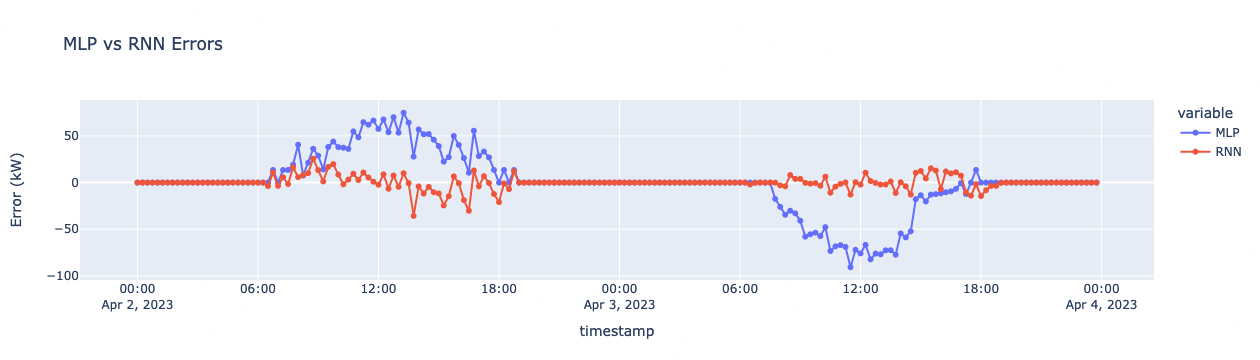
\includegraphics[width=.9\textwidth]{chapters/4_evaluation/imgs/mlpvsrnn/mlpvsrnn1.png}
		\caption{}
	\end{subfigure}
	\begin{subfigure}{\textwidth}
		\centering
		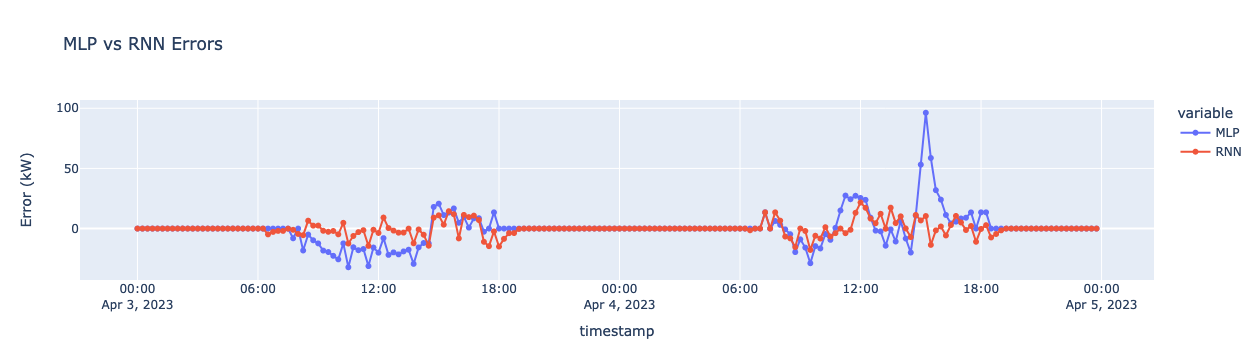
\includegraphics[width=.9\textwidth]{chapters/4_evaluation/imgs/mlpvsrnn/mlpvsrnn2.png}
		\caption{}
	\end{subfigure}
	\begin{subfigure}{\textwidth}
		\centering
		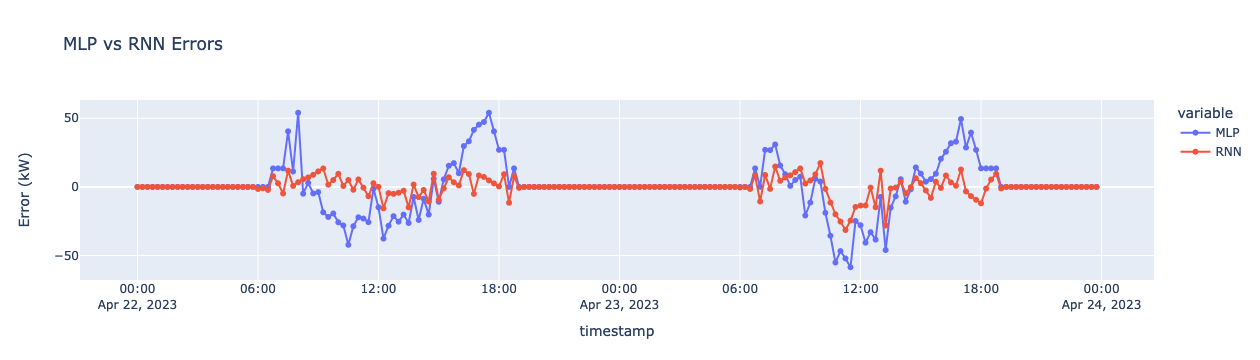
\includegraphics[width=.9\textwidth]{chapters/4_evaluation/imgs/mlpvsrnn/mlpvsrnn3.png}
		\caption{}
	\end{subfigure}
	\caption{Nella figura sono mostrate le curve delle differenze tra target e predizione dei modelli basati su MLP (mostrate in blu) e su RNN (in rosso).}
	\label{fig:mlpvsrnngrafici}
\end{figure}

Dai grafici mostrati in Figura~\ref{fig:mlpvsrnngrafici} possiamo
notare immediatamente che l'architettura che sfrutta le reti ricorrenti
commette errori significativamente più bassi di quella basata su MLP.
Notiamo come le curve in rosso sono generalmente più compatte ed abbastanza
vicine allo 0 (nessun errore commesso). Mentre quelle in blu s

\begin{table}[H]
	\centering
	\begin{tabular}{l|l|l|l|l}
		\multicolumn{1}{c|}{\textbf{Gap}} &
		\makecell{\textbf{MLP MAE}                                       \\\textbf{(kW)}} &
		\textbf{\makecell{RNN MAE                                        \\(kW)}} &
		\textbf{\makecell{Diff                                           \\(kW)}}  &
		\textbf{\makecell{Diff                                           \\(\%)}}  \\ %% ((MLP - RNN)*100)/MLP
		\hline
		02-04 to 03-04                    & 18.63 & 3.91 & 14.72 & 79.01 \\
		03-04 to 04-04                    & 06.90 & 3.29 & 03.61 & 52.31 \\
		04-04 to 05-04                    & 10.41 & 5.55 & 04.86 & 46.68 \\
		05-04 to 06-06                    & 17.99 & 6.89 & 11.10 & 61.70 \\
		06-04 to 07-04                    & 20.07 & 6.78 & 13.29 & 66.21 \\
		07-04 to 08-04                    & 14.77 & 9.25 & 5.52  & 37.37 \\
		08-04 to 09-04                    & 15.82 & 7.85 & 7.97  & 50.39 \\
		09-04 to 10-04                    & 10.30 & 5.82 & 4.48  & 43.49
	\end{tabular}
	\caption{In questa tabella viene messo in evidenza la differenza tra l'errore del modello basato su MLP e quello su Reti Ricorrenti. La colonna \texttt{Diff (kW)} è la differenza in valore assoluto tra MLP MAE e RNN MAE, mentre \texttt{Diff (\%)} è la differenza in percentuale.}
	\label{tab:mlpvsrnndiff}
\end{table}